\documentclass[11pt, twoside, pdftex]{article}

% This includes all the settings that we should use for the document
\newcommand{\PDFTitle}{Introduction to the ARM* Processor \\
Using Intel\textsuperscript{\textregistered} FPGA Toolchain}
\newcommand{\commonPath}{../../Common}
\newcommand{\datePublished}{Mar 2022}

\newcommand{\versnum}{21.1} %version number quartus/AMP
\newcommand{\quartusname}{Quartus\textsuperscript{\textregistered} Prime}	
\newcommand{\textBar}{For \quartusname{} \versnum{}}
\newcommand{\thisyear}{2022 } %for copyright
\newcommand{\company}{FPGAcademy.org}
\newcommand{\longteamname}{FPGAcademy.org}
\newcommand{\teamname}{FPGAcademy}
\newcommand{\website}{FPGAcademy.org}

\newcommand{\productAcronym}{AMP}
\newcommand{\productNameShort}{Monitor Program}

\newcommand{\productNameMedTM}{Monitor Program}
\newcommand{\productNameMed}{Monitor Program}

%\newcommand{\headerLogoFilePath}[1]{#1/FPGAcademy.png}



\setlength\topmargin{-0.25in}
\setlength\headheight{0in}
\setlength\headsep{0.35in}
\setlength\textheight{8.5in}
\setlength\textwidth{7in}
\setlength\oddsidemargin{-0.25in}
\setlength\evensidemargin{-0.25in}
\setlength\parindent{0.25in}
\setlength\parskip{0in} 

\pdfpagewidth 8.5in
\pdfpageheight 11in

% listings is a package that supports encapsulating source code in LaTeX conveniently

\usepackage{listings}
% add support for graphics
\usepackage{graphicx}
\usepackage[usenames, dvipsnames]{color}

\def\expandparam\lstinputlisting[#1]#2{\edef\tmp{\noexpand\lstinputlisting[#1]{#2}}\tmp}

\widowpenalty 10000
\clubpenalty 10000

%%%%%%%%%%%%%%%%%%%% Source Code Formatting %%%%%%%%%%%%%%%%%%%%
\definecolor{globalCommentColour}{rgb}{0.588,0.588,0.588}

%%%%%%%%%%%%%%%%%%%%%%%%%%%%%%%%%%%%%%%%%%%%%%%%%%%%
% Defining a NiosII ASM highlighter for lstlisting
\lstdefinelanguage[NiosII]{Assembler} {
 	morekeywords={add, addi, and, andhi, andi, beq, bge, bgeu, bgt, bgtu, ble,  bleu, blt, bltu, bne, br, break,% 
 	bret, call, callr, cmpeq, cmpeqi, cmpge, cmpgei, cmpgeu, cmpgeui, cmpgt, cmpgti, cmpgtu, cmpgtui, cmple,%
 	cmplei, cmpleu, cmpleui, cmplt, cmplti, cmpltu, cmpltui, cmpne, cmpnei, custom, div, divu, eret, flushd,%
 	flushda, flushi, flushp, initd, initda, initi, jmp, jmpi, ldb, ldbio, ldbu, ldbuio, ldh, ldhio, ldhu, ldhuio,%
 	ldw, ldwio, mov, movhi, movi, movia, movui, mul, muli, mulxss, mulxsu, mulxuu, nextpc, nop, nor, or, orhi, ori,%
 	rdctl, rdprs, ret, rol, roli, ror, sll, slli, sra, srai, srl, srli, stb, stbio, sth, sthio, stw, stwio,%
 	sub, subi, sync, trap, wrctl, wrtcl, wrprs, xor, xori, xorhi, xori},% 	
 	morekeywords=[2]{.abort, .ABORT, .align, .app-file, .ascii, .asciz, .balign, .byte, .comm, .data, .def,%
 	.desc, .dim, .double, .eject, .else, .end, .endef, .endif, .equ, .equiv, .err, .extern, .file, .fill, .float,%
 	.global, .globl, .hword, .ident, .if, .include, .int, .irp, .irpc, .lcomm, .lflags, .line, .linkonce, .ln,%
 	.list, .long, .macro, .mri, .nolist, .octa, .org, .p2align, .psize, .quad, .rept, .sbttl, .scl, .section,%
 	.set, .short, .single, .size, .sleb128, .skip, .space, .stadb, .stabn, .stabs, .string, .symver, .tag,%
 	.text, .title, .type, .val, .uleb128, .word},% 	
 	morekeywords=[3]{et, bt, gp, sp, fp, ea, sstatus, ra, pc, status, estatus, bstatus, ienable, ipending, cpuid,%
 	exception, pteaddr, tlbacc, tlbmisc, eccinj, badaddr, config, mpubase, mpuacc},% 	
 	sensitive=t,%
 	alsoletter=.,%
	morestring=[b]",%
 	morecomment=[s]{/*}{*/},%
 	morecomment=[l]\#,%
   }[keywords,comments,strings]
   
   %% NOTE: morekeywords=[2] are GNU directives.
   
   \definecolor{niosInstructionColour}{rgb}{0.000,0.608,0.000}
   \definecolor{niosDirectiveColour}{rgb}{0.000,0.000,0.902}
   \definecolor{niosSpecialRegColour}{rgb}{0.000,0.000,0.000}
   \definecolor{niosStringColour}{rgb}{0.808,0.482,0.000}
   
   %% NOTE: To make bold use: =\bfseries\color{<colour>}
   \lstdefinestyle{defaultNiosStyle} {
   language=[NiosII]{Assembler},
   stringstyle=\color{niosStringColour},
   keywordstyle=\color{niosInstructionColour},
   keywordstyle=[2]\color{niosDirectiveColour},
   keywordstyle=[3]\itshape\color{niosSpecialRegColour}
   }
%%%%%%%%%%%%%%%%%%%%%%%%%%%%%%%%%%%%%%%%%%%%%%%%%%%%

%%%%%%%%%%%%%%%%%%%%%%%%%%%%%%%%%%%%%%%%%%%%%%%%%%%%
% Defining a ArmA9 ASM highlighter for lstlisting
\lstdefinelanguage[ArmA9]{Assembler} {
 	morekeywords={ADC, ADD, ADDS, AND, ANDS, B, BAL, BEQ, BGE, BGT, BL, BLT, BIC, BKPT, BLX, BNE, BX, CDP, CLZ, CMN, CMP, EOR,%
 	EORS, LDC, LDM, LDR, LDRB, LDRBT, LDRH, LDRSB, LDRSH, LDRT, LSL, MCR, MLA, MOV, MOVW, MOVT, MRC, MRS, MSR, MUL, MVN, ORR, PLD,%
 	ROR, RSB, RSC, SBC, SMLAL, SMULL, STC, STM, STR, STRB, STRBT, STRH, STRT, SUB, SUBS, SWI, SWP, SWPB, TEQ, UMLAL,
 	PUSH, POP, MOVS, RORS, LSR},%
 	morekeywords=[2]{.abort, .ABORT, .align, .app-file, .ascii, .asciz, .balign, .byte, .comm, .data, .def,%
 	.desc, .dim, .double, .eject, .else, .end, .endef, .endif, .equ, .equiv, .err, .extern, .file, .fill, .float,%
 	.global, .globl, .hword, .ident, .if, .include, .int, .irp, .irpc, .lcomm, .lflags, .line, .linkonce, .ln,%
 	.list, .long, .macro, .mri, .nolist, .octa, .org, .p2align, .psize, .quad, .rept, .sbttl, .scl, .section,%
 	.set, .short, .single, .size, .sleb128, .skip, .space, .stadb, .stabn, .stabs, .string, .symver, .tag,%
 	.text, .title, .type, .val, .vectors, .uleb128, .word},%
 	morekeywords=[3]{SP, PC, MIDR, CTR, TCMTR, TLBTR, MPIDR, ID_PFR0, ID_PFR1, ID_DFR0, ID_MMFR0, ID_MMFR1, ID_MMFR2,%
 	ID_MMFR3, ID_ISAR0, ID_ISAR1, ID_ISAR2, ID_ISAR3, ID_ISAR4, CCSIDR, CLIDR, AIDR, CSSELR, TTBR0, TTRB1, TTBR2, DACR,%
 	DFSR, IFSR, ADFSR, AIFSR, DFAAR, IFAR, ICIALLUIS, BPIALLIS, PAR, ICIALLU, ICIMVAU, BPIALL, DCIMVAC, DCISW, V2PCWPR,%
 	DCCVAC, DCCSW, DDIMVAC, DCISW, TLBALLIS, TLBIMVAIS, TLBIASIDIS, TLBIMVAAIS, TLBIALL, TLBIMVA, TLBIASID, TLBIMVAA,%
 	PMCR, PMCNTENSET, PMCNTENCLR, PMOVSR, PMSWINC, PMSELR, PMXEVTYPER, PMXEVCNTR, PMUSERENR, PMINTENSET, PMINTENCLR,%
 	PRRR, NRRR, PLEIDR, PLEASR, PLEFSR, PLEUAR, PLEPCR, VBAR, MVBAR, ISR, FCSEIDR, CONTEXTIDR, TPIDRURW, TPIDRURO, TPIDRPRW},%
 	sensitive=f,%
 	alsoletter=.,%
	morestring=[b]",%
 	morecomment=[s]{/*}{*/},%
 	morecomment=[l]{//},%
   }[keywords,comments,strings]
   
   %% NOTE: morekeywords=[2] are GNU directives.
   
   \definecolor{armInstructionColour}{rgb}{0.000,0.608,0.000}
   \definecolor{armDirectiveColour}{rgb}{0.000,0.000,0.902}
   \definecolor{armSpecialRegColour}{rgb}{0.000,0.000,0.000}
   \definecolor{armStringColour}{rgb}{0.808,0.482,0.000}
   
   \lstdefinestyle{defaultArmStyle} {
   language=[ArmA9]{Assembler},
   stringstyle=\color{armStringColour},
   keywordstyle=\color{armInstructionColour},
   keywordstyle=[2]\color{armDirectiveColour},
   keywordstyle=[3]\itshape\color{armSpecialRegColour}
   }
%%%%%%%%%%%%%%%%%%%%%%%%%%%%%%%%%%%%%%%%%%%%%%%%%%%%

%%%%%%%%%%%%%%%%%%%%%%%%%%%%%%%%%%%%%%%%%%%%%%%%%%%%
% Defining style for the verilog.

\definecolor{verilogCommentColour}{rgb}{0.000,0.502,0.000}

\lstdefinestyle{defaultVerilogStyle} {
language={Verilog},
keywordstyle=\color{blue},
commentstyle=\color{verilogCommentColour}
}
%%%%%%%%%%%%%%%%%%%%%%%%%%%%%%%%%%%%%%%%%%%%%%%%%%%%

%%%%%%%%%%%%%%%%%%%%%%%%%%%%%%%%%%%%%%%%%%%%%%%%%%%%
% Defining style for the vhdl.
\lstdefinestyle{defaultVHDLStyle} {
language={VHDL},
keywordstyle=\color{blue},
commentstyle=\color{verilogCommentColour}
}
%%%%%%%%%%%%%%%%%%%%%%%%%%%%%%%%%%%%%%%%%%%%%%%%%%%%

%%%%%%%%%%%%%%%%%%%%%%%%%%%%%%%%%%%%%%%%%%%%%%%%%%%%
% Java
\definecolor{javaStringColour}{rgb}{0.808,0.482,0}
%%%%%%%%%%%%%%%%%%%%%%%%%%%%%%%%%%%%%%%%%%%%%%%%%%%%

%%%%%%%%%%%%%%%%%%%%%%%%%%%%%%%%%%%%%%%%%%%%%%%%%%%%
% Defining language styles
% C
\definecolor{CStringColour}{rgb}{0.808,0.482,0}
%%%%%%%%%%%%%%%%%%%%%%%%%%%%%%%%%%%%%%%%%%%%%%%%%%%%

%%%%%%%%%%%%%%%%%%%%%%%%%%%%%%%%%%%%%%%%%%%%%%%%%%%%
% Defining extended LaTeX language.
\lstdefinelanguage[LocalLaTeX]{TeX}[LaTeX]{TeX}%
 	{moretexcs={bf, it, sf, lstset},%
   	}%

\lstdefinestyle{defaultLocalLatexStyle} {
language=[LocalLatex]{TeX},
keywordstyle=\color{blue}\bfseries,
keywordstyle=[2]\color{blue},
keywordstyle=[3]\color{blue}\bfseries
}
%%%%%%%%%%%%%%%%%%%%%%%%%%%%%%%%%%%%%%%%%%%%%%%%%%%%

\lstset{
%language = C,
%language = Verilog,
%basicstyle=\color{black}\rmfamily\ttfamily,
basicstyle=\small\color{black}\ttfamily,
commentstyle=\small\color{globalCommentColour}\itshape\ttfamily,
keywordstyle=\small\color{blue}\bfseries\ttfamily,
showstringspaces=false,
frame=none, %lines % boxed listings
breaklines=true,
breakatwhitespace=true,
tabsize=4
}
%%%%%%%%%%%%%%%%%%%%%%%%%%%%%%%%%%%%%%%%%%%%%%%%%%%%%%%%%%%%%%%%


%\usepackage[centering]{geometry}.
%%%%%%%%%%%%%%%%%%%%%%%%%%%%%%%%%%%%%%%%%%%%%%%%%%%
% Document Settings
\usepackage[labelsep=period]{caption}
% we can choose a better font later
%\usepackage{palatino}
\usepackage{fourier}
%\fontencoding{T1}
% include common used symbols
\usepackage{textcomp}
% add support for graphics
\usepackage{graphicx}
\usepackage[usenames, dvipsnames]{color}
% enable to draw thick or thin table hlines
\setlength{\doublerulesep}{\arrayrulewidth}
\usepackage{longtable}
\setlongtables
%\usepackage{array}
% It may be better to use PDFLaTeX as it can generate bookmarks for the
% document

% Add some useful packages
\usepackage{ae,aecompl}
\usepackage{epsfig,float,times}

% reset the font for section
\usepackage{sectsty}
%\allsectionsfont{\fontfamily{ptm}\selectfont}
\allsectionsfont{\usefont{OT1}{phv}{bc}{n}\selectfont}

% use compact space for sections
\usepackage[compact]{titlesec}
\titlespacing{\section}{0pt}{0.2in}{*0}
\titlespacing{\subsection}{0pt}{0.1in}{*0}
\titlespacing{\subsubsection}{0pt}{0.05in}{*0}

% fancyhdr header and footer customization
\usepackage{layout}
\usepackage{fancyhdr}
\pagestyle{fancy}
\fancyhead{}
\fancyhead[R]{\textit{\tiny{\textBar}}}
\fancyfoot{}
\fancyfoot[LO,
RE]{\textrm{\href{https://www.fpgacademy.org}{\small \longteamname}} \\ {\small \datePublished }}
\fancyfoot[RO, LE]{\small \thepage}
% two-side settings
%\fancyhead{} % clear all header fields
%\fancyfoot{} % clear all footer fields
%\fancyfoot[LE,RO]{\thepage}
\renewcommand{\headrulewidth}{2pt}
\renewcommand{\headrule}{{\color{blue} \hrule width\headwidth height\headrulewidth \vskip-\headrulewidth}}
\renewcommand{\footrulewidth}{0pt}

% Format the footer on page 1
\fancypagestyle{plain}{
\fancyhead{}
\fancyfoot{}
\fancyfoot[LO,
RE]{\textrm{\href{https://www.fpgacademy.org}{\small \longteamname}} \\ {\small \datePublished }}
\fancyfoot[RO, LE]{\small \thepage}
\renewcommand{\headrulewidth}{0pt}
}
% adjust some setting to try to make the figure stay in the same page with text
% Reference: 	http://www.cs.uu.nl/~piet/floats/node1.html
%   			http://mintaka.sdsu.edu/GF/bibliog/latex/floats.html
%   General parameters, for ALL pages:
\renewcommand{\topfraction}{0.9}	% max fraction of floats at top
\renewcommand{\bottomfraction}{0.8}	% max fraction of floats at bottom
%   Parameters for TEXT pages (not float pages):
\setcounter{topnumber}{3}
\setcounter{bottomnumber}{3}
\setcounter{totalnumber}{5}     % 2 may work better
\setcounter{dbltopnumber}{2}    % for 2-column pages
\renewcommand{\dbltopfraction}{0.9}	% fit big float above 2-col. text
\renewcommand{\textfraction}{0.07}	% allow minimal text w. figs
%   Parameters for FLOAT pages (not text pages):
\renewcommand{\floatpagefraction}{0.7}	% require fuller float pages
% N.B.: floatpagefraction MUST be less than topfraction !!
\renewcommand{\dblfloatpagefraction}{0.7}	% require fuller float pages
%%%%%%%%%%%%%%%%%%%%%%%%%%%%%%%%%%%%%%%%%%%%%%%%%%%
% remember to use [htp] or [htpb] for placement
%%%%%%%%%%%%%%%%%%%%%%%%%%%%%%%%%%%%%%%%%%%%%%%%%%%

% set no indent for paragraph
\setlength{\parindent}{0em}
\addtolength{\parskip}{11pt}
\newcommand{\compact}{[topsep=0pt]}
% use this package to reduce space
\usepackage{enumitem}
\usepackage{multirow}
\usepackage{rotating}
\usepackage{pifont}
\usepackage{dingbat}
\newcommand{\itemsecond}{$\circ$}
%
%%%%%%%%%%%%%%%%%%
\date{}
\author{}
%%%%%%%%%%%%%%%%%%
\newcommand{\de}{DE-series}
\newcommand{\up}{FPGAcademy}
\newcommand{\fabric}{Avalon Switch Fabric}
\newcommand{\TODO}[1]{\textcolor{red}{\textbf{TODO}: #1}}
\def\registered{{\ooalign{\hfil\raise .00ex\hbox{\scriptsize R}\hfil\crcr\mathhexbox20D}}}

% enable url and reference(bookmarks) in pdf
\usepackage{url}
\usepackage[pdftex, colorlinks]{hyperref}
\hypersetup{%
pdftitle={\PDFTitle},
linkcolor=blue,
hyperindex=true,
pdfauthor={\longteamname},
pdfkeywords={FPGAcademy, Academic Program, Example System},
bookmarksnumbered,
bookmarksopen=false,
filecolor=blue,
pdfstartview={FitH},
urlcolor=blue,
plainpages=false,
pdfpagelabels=true,
linkbordercolor={1 1 1} %no color for link border
}%
%%%%%%%%%%%%%%%%%%%%%%%%%%%%%%%%%%%%%%%%%%%%%%%%%%%
\setlength{\fboxsep}{0.7pt}
\setlength{\fboxrule}{0.5pt}

\newcommand{\red}[1]{{\color{red}\sf{#1}}}
\newcommand{\blue}[1]{{\color{blue}\sf{#1}}}



%%%%%%%%%%%%%%%%%%%%%%%%%
% Add title
\newcommand{\doctitle}{Introduction to the 
ARM* Processor \\ Using
Intel\textsuperscript{\textregistered} FPGA Toolchain}
\newcommand{\dochead}{Introduction to the
ARM* Processor Using Intel\textsuperscript{\textregistered} FPGA
Toolchain}
% Usually no need to change these two lines
\title{\fontfamily{phv}\selectfont{\doctitle} }
\chead{ \small{\textsc{\bfseries \dochead} } }
% Customizations
%%%%%%%%%%%%%%%%%%%%%%%%%
% Allows multiple figures per page

\renewcommand\floatpagefraction{.9}
\renewcommand\topfraction{.9}
\renewcommand\bottomfraction{.9}
\renewcommand\textfraction{.1}   
\setcounter{totalnumber}{50}
\setcounter{topnumber}{50}
\setcounter{bottomnumber}{50}
\raggedbottom

%%%%%%%%%%%%%%%%%%
%%% DOCUMENT START
%\begin{document}
\begin{document}
\begin{table}
    \centering
    \begin{tabular}{p{5cm}p{4cm}}
        \hspace{-3cm}
        &
        \raisebox{1\height}{\parbox[h]{0.5\textwidth}{\Large\fontfamily{phv}\selectfont{\textsf{\doctitle}}}}
    \end{tabular}
    \label{tab:logo}
\end{table}

\colorbox[rgb]{0,0.384,0.816}{\parbox[h]{\textwidth}{\color{white}\textsf{\textit{\textBar}}}}

\thispagestyle{plain}
 
\section{Introduction}
\label{sec:intro}

This tutorial presents an introduction to the 
ARM Cortex-A9* processor, 
which is a processor implemented as a hardware block in the Intel\textsuperscript{\textregistered}
Cyclone\textsuperscript{\textregistered} V SoC FPGA devices.
The tutorial is intended for a user who wishes to use an
ARM-based system on Intel's DE1-SOC board.

A full description of ARM processors is provided in the 
{\it ARM Architecture Reference Manual}, which is available on the ARM Holdings web site. 

{\bf Contents}:
\begin{itemize}
\item Overview of ARM Cortex-A9 Processor Features
\item Register Structure
\item Instruction Sets
\item Accessing Memory and I/O Devices
\item Addressing Modes
\item ARM Instructions
\item Assembler Directives
\item Example Program
\item Operating Modes
\item Banked Registers
\item Exception Processing
\item Input/Output Operations
\end{itemize}
\clearpage
\newpage

\section{Overview of ARM Cortex-A9* Processor Features}
The ARM Cortex-A9 processor has mostly a Reduced Instruction Set Computer (RISC) architecture.
Its arithmetic and logic operations are performed on operands in the general-purpose
registers. The data is moved between the memory and these registers by means of {\it Load}
and {\it Store} instructions.

The word-length of the processor is 32 bits. Data byte addresses in a 32-bit word 
are assigned in {\it little-endian} style, 
in which the lower byte addresses are used for the less
significant bytes (the rightmost bytes) of the word. 

\section{Register Structure}
All registers in the ARM Cortex-A9 processor are 32 bits long.
There are 15 general-purpose registers, R0 to R14,
a Program Counter, R15, and a Current Program Status
Register, CPSR, as shown in Figure 1.
All general-purpose registers can be used in the same way. 
However, software programs usually treat two of them in a special 
way. Register R13 is used as a Stack Pointer.
Register R14 is used as a Link Register in subroutine linkage.
In assembly-language programs, the registers
R15, R14 and R13 can also be referred to by using the acronyms
PC, LR and SP, respectively. In assembly-language programs, the
register names can be written either in upper or lower case.
Thus, R1, R2, PC, LR and SP is equivalent to r1, r2, pc, lr and
sp.

\begin{figure}[H]
   \begin{center}
      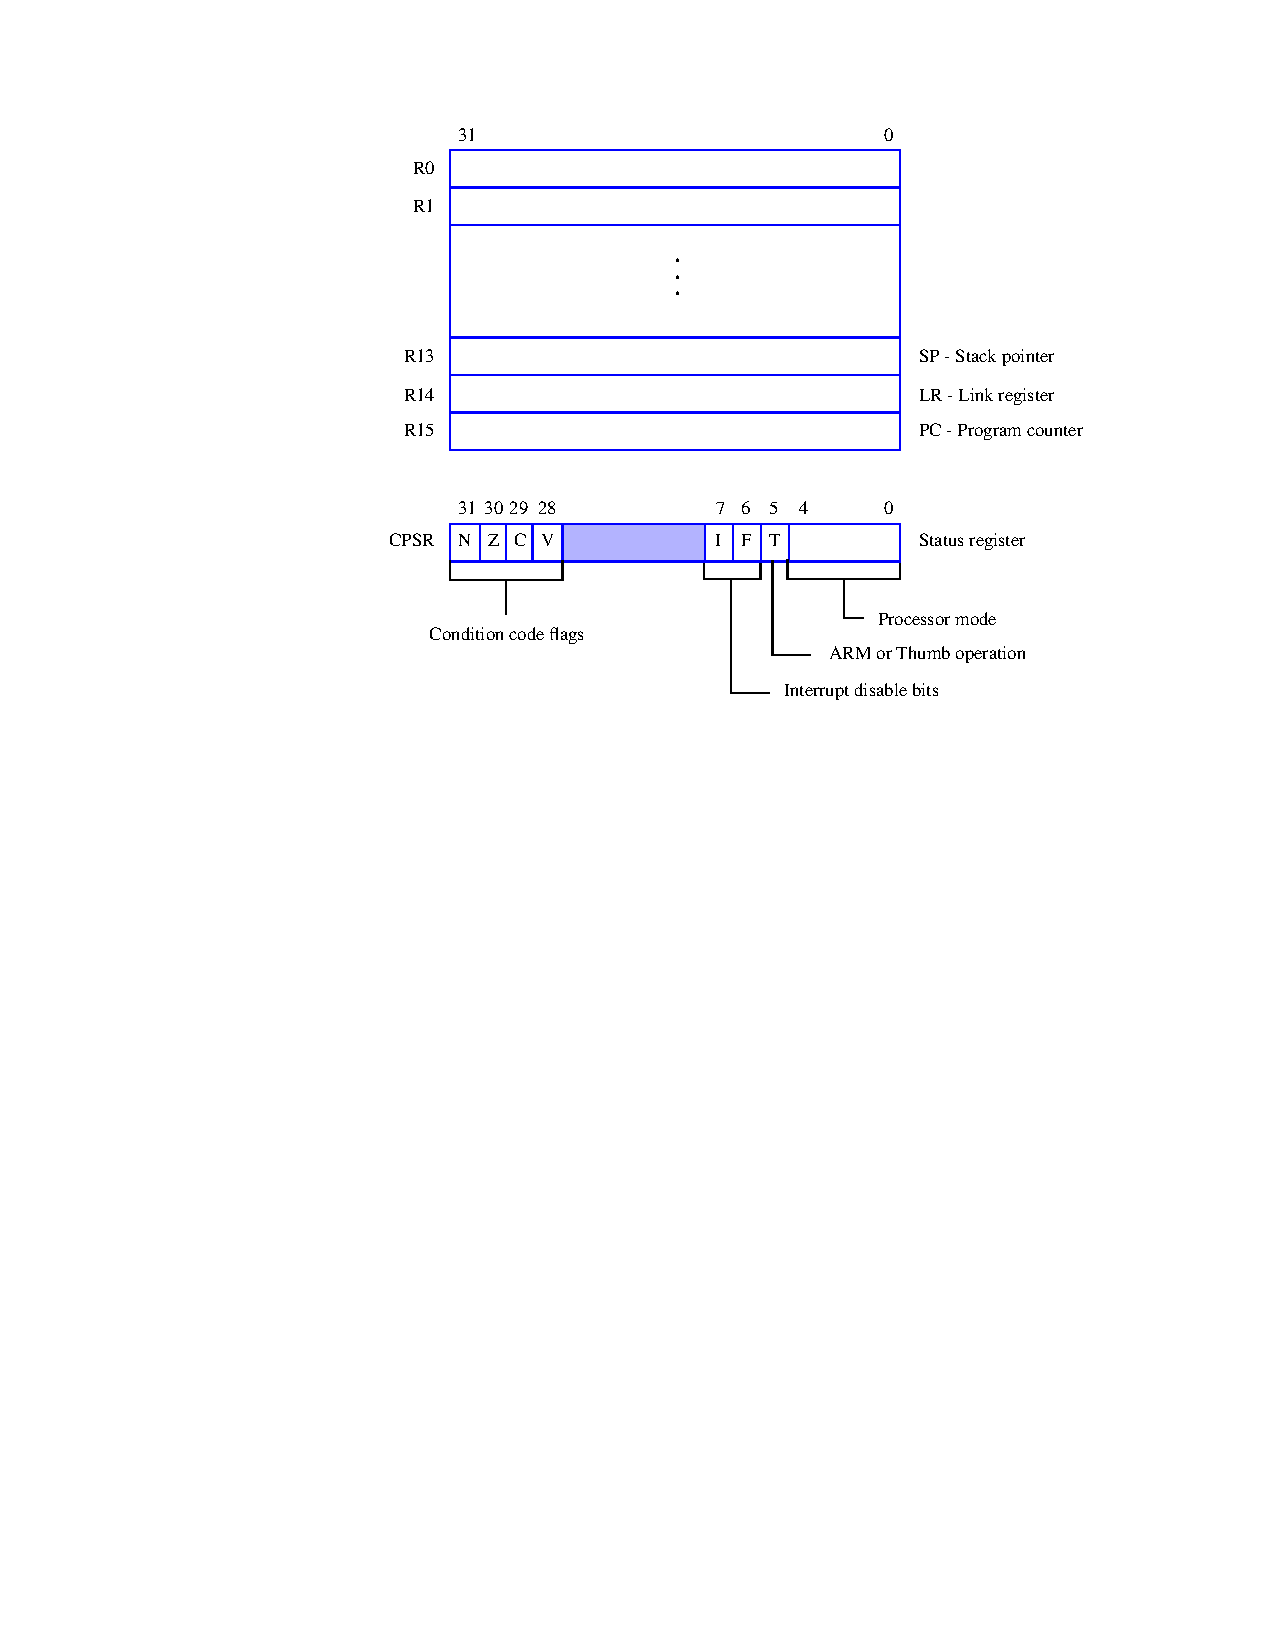
\includegraphics[scale=1]{figures/figure1.pdf}
   \caption{ARM register structure.} 
	 \label{fig:1}
	 \end{center}
\end{figure}

The CPSR register has the following contents:
\begin{itemize}
\item Condition Code flags which are set based on the results
of a previous operation. Most ARM instructions can be executed
conditionally based on the values of these flags:
\begin{itemize}
\item Negative (N) - set to 1 if the result is negative;
otherwise, cleared to 0
\item Zero (Z) - set to 1 if the result is 0; otherwise,
cleared to 0.
\item Carry (C) - set to 1 if a carry-out results from the
operation; otherwise, cleared to 0.
\item Overflow (V) - set to 1 if arithmetic overflow occurs;
otherwise cleared to 0.
\end{itemize}
\item Interrupt-disable bits, I and F, where
\begin{itemize}
\item I = 1 disables the IRQ interrupts
\item F = 1 disables FIQ interrupts
\end{itemize}
\item Thumb bit, where
\begin{itemize}
\item T = 0 indicates ARM execution
\item T = 1 indicates Thumb execution
\end{itemize}
\item Processor mode bits which identify the mode in which
the processor is operating, as explained in Section 9.
\end{itemize}
 
For some registers, there are duplicate registers, called
{\it banked} registers, for saving 
the contents of primary registers when various types of
interrupts occur, as discussed in Section 10.

\section{Instruction Sets}
\label{sec:inst}

The ARM Cortex-A9 processor can execute instructions in three
different instruction sets, known as ARM, Thumb* and Thumb*-2.

The ARM set is the most powerful. All instructions
are 32 bits long. The instructions are stored in memory in
word-aligned manner.

The Thumb set is a smaller version, where the 
instructions are provided in a format that uses only 16 bits.
This usually results in smaller memory requirements, which can be
useful in embedded applications.

The Thumb-2 set includes both 16- and 32-bit instructions.
Its functionality is almost identical to that of the ARM
instruction set.

In this tutorial we will deal only with the ARM instruction set.
We should note that there exists a {\it Unified Assembler
Language (UAL)}, which provides a common syntax for ARM and
Thumb instructions. It supersedes the previous versions of
both the ARM and Thumb assembler languages. We will use UAL
in this tutorial. 

\section{Accessing Memory and I/O Devices}
\label{sec:mem_IO}

Any input/output devices that can be accessed by the ARM
processor are memory mapped and can be accessed as memory
locations. Data accesses to memory locations and I/O interfaces
are performed by means of Load and Store instructions, which cause data 
to be transferred between the memory and
general-purpose registers.
The ARM processor issues 32-bit addresses. The memory space is byte-addressable. 
Instructions can read and write {\it words} 
(32 bits), {\it halfwords} (16 bits), or {\it bytes} (8 bits) of data.

\subsection{Addressing Modes for Load and Store Instructions}
\label{sec:modes}

The Load and Store instructions are the only type of instructions
that can access memory locations.
Load instructions copy the contents of a memory location
specified by an addressing mode into a destination register,
which is a general-purpose register, R$d$.
Store instructions copy the contents of a general-purpose
register, R$d$, into a memory location specified by an
addressing mode.

An addressing mode provides the information needed to determine the address of the desired memory location. 
There are different ways of specifying the required address. 
All addressing modes involve one or two
general-purpose registers, plus some additional information.
One register is referred to as the {\it base} register, R$n$.
If a second register is used, it is referred to as the
{\it index} register, R$m$. The memory address is determined by
adding the contents of the base register and a value that is
either given as a signed 12-bit {\it offset} directly in the
instruction or as a magnitude in the index register.
The magnitude in R$m$ can be scaled by shifting it either left
or right a number of bit-positions specified in the instruction.

There are three primary addressing modes provided:
\begin{itemize}
\item {\it Offset} mode -- the address is determined by adding
the contents of a base register and an offset that is either
given directly in the instruction or in an index register.
\item {\it Pre-indexed} mode -- the address is determined
in the same way as in the Offset mode; subsequently, this
address replaces the contents of the base register used. 
\item {\it Post-indexed} mode -- the address is the contents
of a base register; subsequently, the base register is loaded
with a new address that is determined in the same way as in
the Offset mode.
\end{itemize}

\noindent
These addressing modes are fully specified in Table 1, 
which indicates how the address generation is performed.
The table also gives the required Assembler syntax.

When an index register is specified, its contents are interpreted
as a magnitude which can be either added to or subtracted from 
a base register. This magnitude can first be shifted left or
right by specifying LSL \#k or LSR \#k, respectively, where k
is an integer from 1 to 31. Shifting operations are discussed further in 
section \ref{sec:shifts}.

Since the Program Counter, R15, can be treated as a
general-purpose register, it can be used in the Offset
addressing mode as a base register, R$n$. This makes it possible
to access memory locations in terms of their 
distance relative to the current address in R15.
This mode is often referred to as the {\it Relative} addressing
mode. 

\newpage
\begin{center}
{\bf TABLE 1. ~Memory addressing modes }
~\\
\begin{tabular}{@{}lll@{}} \hline
&& \\ [-1ex]
{\bf Name} & {\bf Assembler syntax} & {\bf Address generation} \\
&& \\ [-1ex] \hline
&& \\ [-1.5ex]
\multicolumn{3}{@{}l}{Offset:} \\ 
&& \\ [-1ex]
\qquad immediate offset & [R$n$, \#offset] & Address $=$ R$n$ $+$ offset \\
&& \\ [-1ex]
\qquad offset in R$m$ & [R$n$, $\pm$R$m$, shift] &
Address $=$ R$n$ $\pm$ R$m$ shifted \\ 
&&\\ [-1ex]
Pre-indexed:  & & \\
&&\\ [-1ex]
\qquad immediate offset & [R$n$, \#offset]! & Address $=$ R$n$ $+$ offset; \\
           &           & R$n \leftarrow$ address \\
&&\\ [-1ex]
\qquad offset in R$m$ & [R$n$, $\pm$R$m$, shift]! 
& Address $=$ R$n$ $\pm$ R$m$ shifted; \\ 
&  &  R$n \leftarrow$ address \\
&&\\
Post-indexed:  & & \\
&&\\ [-1ex]
\qquad immediate offset & [R$n$], \#offset & Address $=$ R$n$; \\
      &    & R$n \leftarrow$ R$n$ $+$ offset \\
&&\\
\qquad offset in R$m$ & [R$n$], $\pm$R$m$, shift & Address $=$ R$n$; \\
& &  R$n \leftarrow$ R$n$ $\pm$ R$m$ shifted \\
&& \\ [-1.2ex] \hline
\end{tabular}

\smallskip

\begin{tabular}{p{6ex}l@{}}
\multicolumn{2}{l}{offset $=$ a signed number given in the instruction} \\
\multicolumn{2}{l}{shift $\;\,=\;\,$ direction \#integer} \\
& where direction is LSL for left shift or LSR for right shift, and \\
& integer is a 5-bit unsigned  number specifying the shift amount\\
& \\ [-1ex]
\multicolumn{2}{l}{$\pm$R$m$ $=$ the magnitude in register
R$m$ that is added to or subtracted} \\
&  from the contents of base register R$n$ \\
\end{tabular}
\end{center}

Consider the {\it Load} instruction, LDR, which loads a 32-bit operand
into a register. The instruction
\begin{center}
LDR~~~R2, [R6, \#$-$8]
\end{center}
\noindent
loads R2 from the address in R6 minus 8. The instruction
\begin{center}
LDR~~~R2, [R6, \#0x200]
\end{center}
\noindent
loads R2 from the address in R6 plus the hexadecimal number
0x200. The instruction
\begin{center}
LDR~~~R2, [R6, $-$R8]
\end{center}
\noindent
loads R2 from the address obtained by subtracting the contents
of R8 from the contents of R6.

The Pre-indexed mode is illustrated in 
\begin{center}
LDR~~~R2, [R6, R8, LSL \#4]!
\end{center}
\noindent
which loads R2 from the location whose address is determined by
shifting the contents of R8 to the left by 4 bit-positions
(which is equivalent to multiplying by 16) and adding the result
to the contents of R6. Subsequently, the generated address is
loaded into R6.

An example of Post-indexed mode is
\begin{center}
LDR~~~R2, [R6], \#20
\end{center}
\noindent
where R6 contains the address of the location from which an
operand is loaded into R2. Subsequently, the contents of R6
are modified by adding to them the offset value 20.

Relative addressing can be used simply by specifying the address
label associated with the desired memory location. 
For example, if MEMLOC is the desired location, then the
instruction
\begin{center}
LDR~~~R2, MEMLOC
\end{center}
\noindent
will load the contents of memory location MEMLOC into register
R2. The assembler will determine the immediate offset as the
difference between the address MEMLOC and the contents of the
updated Program Counter. It will generate the instruction
\begin{center}
LDR~~~R2, [R15, \#offset]
\end{center}
\noindent
This offset takes into account the fact that when the instruction
is to be executed, the Program Counter will already be
incremented by 8, because the ARM processor will already have fetched the next instruction (due to pipelined execution). 

\subsection{Format for Load and Store Instructions}
\label{sec:machine_code}

The format for Load and Store instructions is shown in Figure 2.
The operation code (OP-code) is provided in bits 27 to 20.
The register R$d$, which is used as the destination in load instructions or as the 
source in store instructions, is
identified by bits 15 to 12.
The base register, R$n$, is identified by bits 19 to 16.
Bits 11 to 0 may contain a signed 12-bit offset or identify
an index register.
If an index register is used, its number, $m$, is given in 
the low-order four bits of the instruction.

Observe, in Figure 2, that the high-order four bits denote a
condition for the instruction. In ARM processors, most
instructions can be executed conditionally, as explained in
Section 6.11.

\begin{figure}[H]
   \begin{center}
      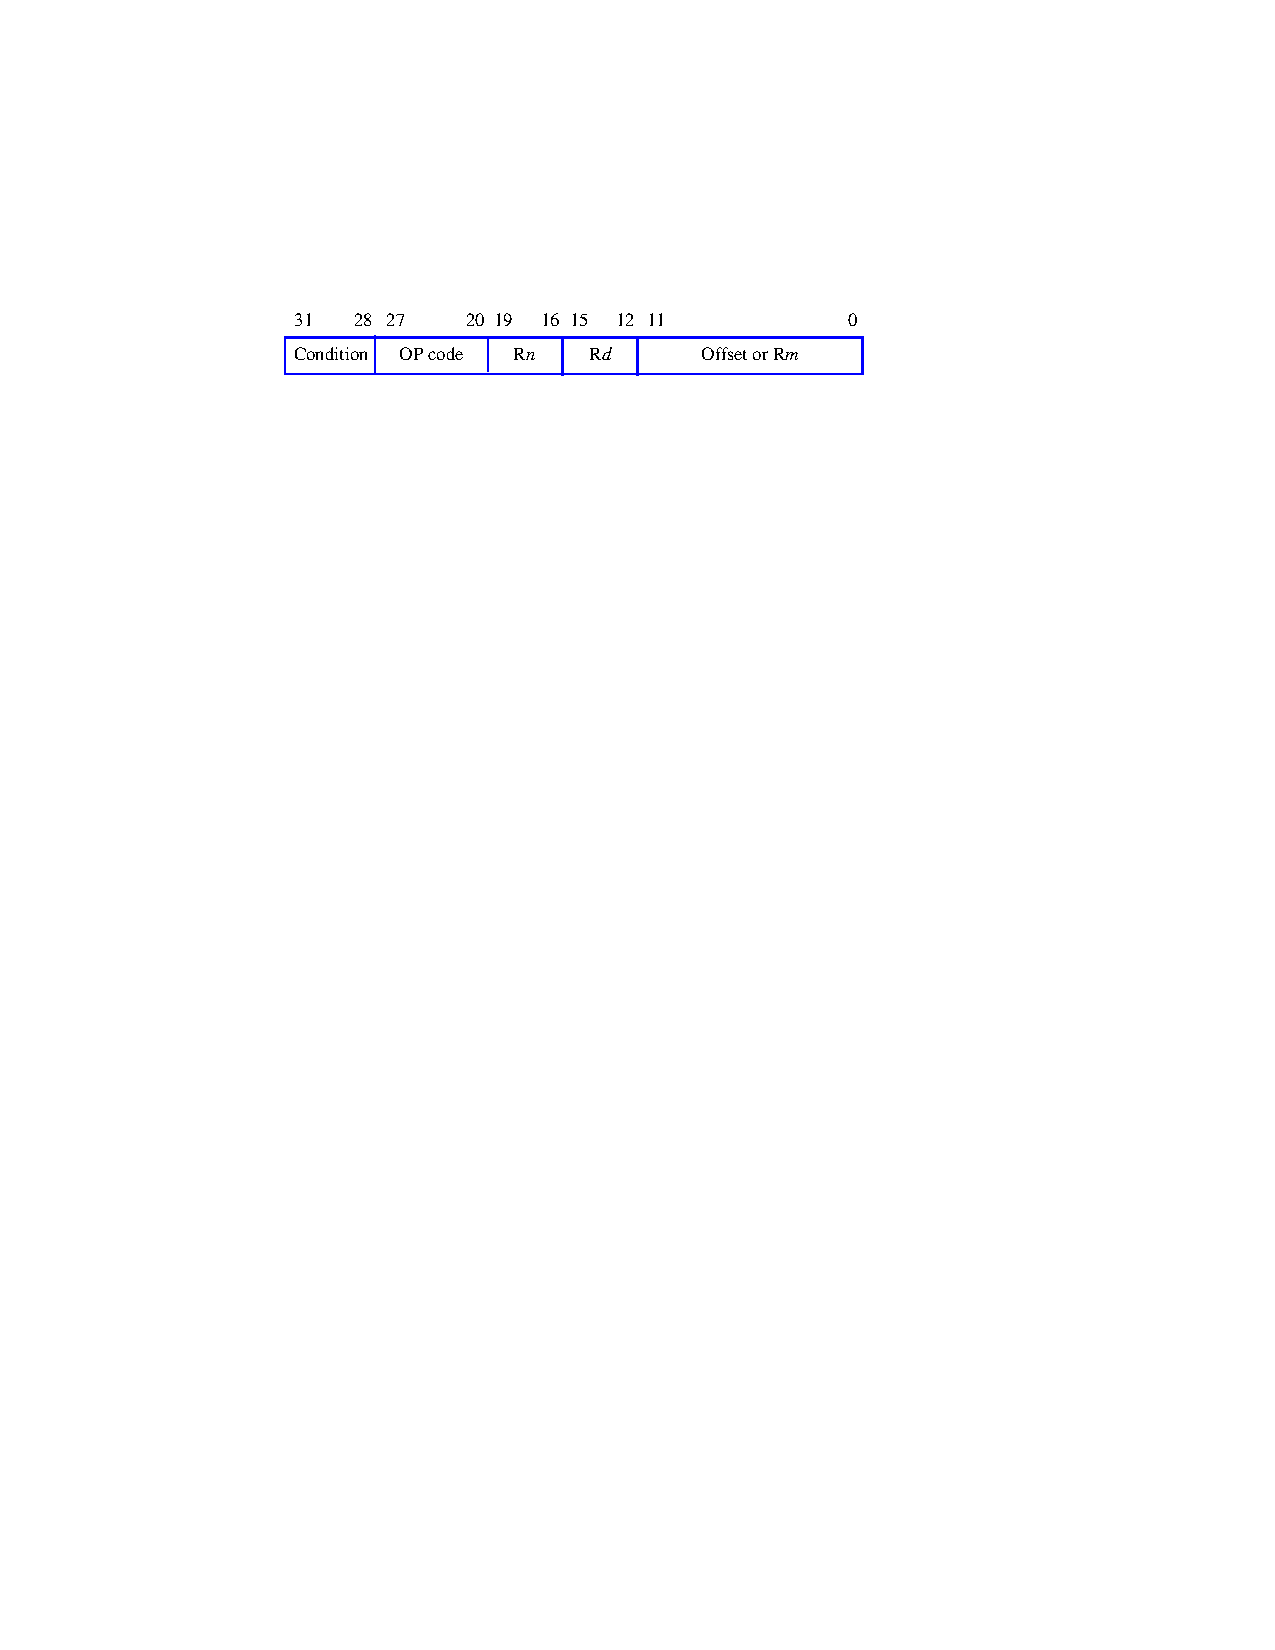
\includegraphics[scale=1]{figures/figure2.pdf}
   \caption{Format for Load and Store instructions.} 
	 \label{fig:2}
	 \end{center}
\end{figure} 

\section{ARM* Instructions}
\label{sec:ARM_inst}

ARM instructions are 32-bits long. In addition to machine instructions that are executed 
directly by the processor, the ARM instruction set includes a number of
{\it pseudo-instructions} that can be used in assembly language
programs. The Assembler replaces each pseudo-instruction by one 
or more machine instructions.

This section discusses briefly the main features of the ARM instruction set. For a complete description of the instruction
set, including the details of how each instruction is encoded,
the reader should consult the 
{\it ARM Architecture Reference Manual}.

\subsection{Load and Store Instructions}
\label{sec:load_store}

Load and store instructions are used to move data between memory
(and I/0 interfaces) and the general-purpose registers. 
The LDR (Load Register) instruction, illustrated in the previous
section, loads a 32-bit operand into a register. 
The corresponding {\it Store} instruction is STR (Store Register). 
For example,
\begin{center}
STR~~~R2, [R4]
\end{center}
\noindent
copies the contents of R2 into memory location at the address
that is found in register R4.

There are also load and store instructions that use operands that are only 8 or 16 bits long.
They are referred to as Load/Store Byte and Load/Store Halfword instructions, respectively.
Such load instructions are: 
\begin{itemize}
\item LDRB~ (Load Register Byte)
\item LDRSB~ (Load Register Signed Byte)
\item LDRH~ (Load Register Halfword)
\item LDRSH (Load Register Signed Halfword)
\end{itemize}
\noindent
When a shorter operand is loaded into a 32-bit register, its value has to be adjusted to fit into the register. This is done by zero-extending the 8- or 16-bit value to 32 bits
in the LDRB and LDRH instructions. In the LDRSB and LDRSH
instructions the operand is sign-extended.
 
The corresponding {\it Store} instructions are: 
\begin{itemize}
\item STRB (Store Register Byte)
\item STRH (Store Register Halfword)
\end{itemize}
\noindent
The STRB instruction stores the low byte of register R$d$ into
the memory byte specified by the address. The STRH instruction
stores the low halfword of register R$d$. 

\subsubsection{Loading and Storing Multiple Registers}
\label{sec:multi}
There are two instructions that allow loading of data into
multiple registers, LDM (Load Multiple), and storing the contents
of multiple registers into memory, STM (Store Multiple).
The memory operands must be in successive word locations.
These instructions are useful for two main purposes:
\begin{itemize}
\item transferring blocks of data between memory and processor
registers, and
\item saving data in registers on a stack, and then later restoring the registers from the stack
\end{itemize}
\noindent
The address of the first word in memory is given in the base
register, R$n$. Upon transferring the last word of data, the
contents of R$n$ can be updated with the last address by
specifying the Pre-indexed (!) addressing mode.

An instruction must specify the registers involved in the
transfer. The registers must be listed in the assembly-language instruction
in a field enclosed by braces, but they
do not have to be contiguous. A range of registers is specified
by listing the first and the last registers in the range,
separated by a dash ($-$). In the resulting machine instruction,
each register is identified by setting a corresponding bit in
the field comprising the low-order 16 bits. Registers are always stored by STM in the order from
largest-to-smallest register-index (R15, R14, R13, $\ldots$, R0), and loaded by LDM in the 
order from the smallest-to-largest register-index (R0, R1, R2, $\ldots$, R15).

The instruction must also indicate the direction in which
memory addresses are computed. For block transfers there are four
possibilities for determining the addresses of consecutive data
words. The address can be incremented or decremented by 4 either before or after each 
data item is accessed. The desired action
is specified by appending a suffix to the OP-code mnemonic in the 
assembly-language instruction. The four suffixes are:
\begin{itemize}
\item IA -- Increment After
\item IB -- Increment Before
\item DA -- Decrement After
\item DB -- Decrement Before
\end{itemize}
\noindent
For example, the instruction
\begin{center}
LDMIA~~R3!, \{R4, R6$-$R8, R10\}
\end{center}
will load registers R4, R6, R7, R8 and R10. If the starting
address in R3 is 1000, then the data loaded into the registers
will be from addresses 1000, 1004, 1008, 1012 and 1016,
respectively. Because the Pre-indexed mode is specified, the
final contents of R3 will be 1020.

The LDM and STM instructions are very useful in the context of
subroutines, where they can be used to save the contents of
registers on the stack. For this purpose, there exist 
pseudo-instructions PUSH and POP, which are actually implemented 
as particular forms of STM and LDM instructions.
In these instructions the Stack Pointer, SP, is the base
register, which is always updated. The SP is decremented by 4
before each transfer in PUSH instructions, and it is incremented
by 4 after each transfer in POP instructions.
For example, the instruction 
\begin{center}
PUSH~~~\{R1, R3$-$R5\}
\end{center}
\noindent
places the contents of registers R5, R4, R3 and R1 onto the stack.
The equivalent {\it Store Multiple} instruction is
\begin{center}
STMDB~~~SP!, \{R1, R3$-$R5\}
\end{center}
\noindent
The instruction
\begin{center}
POP~~~\{R1, R3$-$R5\}
\end{center}
\noindent
restores the contents of these registers from the stack.
The equivalent {\it Load Multiple} instruction would be
\begin{center}
LDMIA~~~SP!, \{R1, R3$-$R5\}
\end{center}
 
\subsection{Data Processing Instructions}
\label{sec:processing}

\noindent
A variety of ARM instructions are provided for the processing of data, including 
instructions that perform shifting, arithmetic operations, logical
operations, and data transfer between registers.

\subsection{Flexible Operands}
\label{sec:operand2}

\noindent
A number of data processing instruction have the general form

\begin{center}
OP~~~~R$d$, R$n$, {\it Operand2}
\end{center}
\noindent
where R$d$ is the destination register, R$n$ is the first operand, and {\it Operand2}
is the second operand. A considerable amount of flexibility is provided by {\it Operand2}.
It can be an immediate constant, as in
\begin{center}
OP~~~~R$d$, R$n$, \#value
\end{center}
\noindent
This instruction performs the operation {\it OP} using the contents of R$n$ and the constant
{\it value}, and places the result into R$d$. For example, if OP is the addition instruction ADD,
then
\begin{center}
ADD~~~R0, R1, \#1
\end{center}
\noindent
adds 1 to the contents of R1 and places the sum into R0. The constant {\it value} can be
specified as a decimal number, as in this example, or as a binary value \#0b1, or as
a hexadecimal value \#0x1. Valid constants include any eight-bit value, such as 0xFF. The
eight-bit value can also be produced by rotation in a 32-bit word---for example, other valid 
constants include 0xFF000000, 0xFF0000, and 0xFF00. In general, the constant can be any 
value which can be generated by rotating a byte to the right any {\it even} number of times
(0, 2, $\ldots$, 30) in a 32-bit word (see the {\it ARM Assembler Reference} for more details).

\noindent
Alternatively, {\it Operand2} can be given as a register R$m$, as in
\begin{center}
OP~~~~R$d$, R$n$, R$m$
\end{center}

\noindent
This instruction performs the operation {\it OP} using the contents of R$n$ and R$m$, and
places the result into R$d$. For example
\begin{center}
ADD~~~R0, R1, R2
\end{center}
\noindent
adds the contents of R1 and R2, and places the sum into R0.

\noindent
When {\it Operand2} is a register, R$m$ can either be used directly, as in the 
above example, or else its value can be shifted before being used. 
If it is shifted, then the shifting amount can be specified as a 
five-bit constant, as in
\begin{center}
OP~~~R$d$, R$n$, R$m$, LSL \#3
\end{center}

\noindent
or as the least-significant byte of a register R$s$, as in
\noindent
\begin{center}
OP~~~R$d$, R$n$, R$m$, LSL R$s$
\end{center}
\noindent
In these examples LSL means {\it Logical Shift Left}. Other examples
of shift variants include right-shift, and rotate operations, as 
discussed in section \ref{sec:shifts}.

\subsubsection{Using Condition Code Flags}
\label{sec:conditions}
The data processing instructions can optionally affect the ARM condition code flags, or
can be executed conditionally based on the values of the condition code flags. These
options are expressed in the general form
\begin{center}
OP\{S\}\{cond\}~~~~R$d$, R$n$, {\it Operand2}
\end{center}
\noindent
If $S$ is included in the instruction mnemonic, as in ADDS, then the condition code flags
will be set depending on the results of the instruction. But if $S$ is not included, as in ADD,
then the flags are unaffected by the instruction. Setting of the condition code flags is
discussed further in Section \ref{sec:CCF}.

\noindent
An optional {\it cond} appended to an instruction mnemonic allows an instruction 
to be either executed or skipped, depending on the current values of the condition code flags. This 
concept is discussed in Section \ref{sec:cond}.

\noindent
\subsection{Arithmetic Instructions}
\label{sec:arith}

As illustrated above, an arithmetic operation such as
\begin{center}
		  ADD~~~R$d$, R$n$, {\it Operand2}
\end{center}
\noindent
adds the contents of R$n$ and the value
determined as {\it Operand2} into R$d$. For example, the instruction
\begin{center}
ADD~~~R0, R1, R2, LSL \#2
\end{center}
\noindent
adds the contents of R1 and a shifted version of the contents of
R2, and places the sum into R0. The operand R2 is shifted to the left by 2 bit
positions (which is equivalent to integer multiplication by 4)
before it is used in the addition. 

\noindent
In an assembly-language instruction, it is possible to specify
a negative number as the immediate operand, as in
\begin{center}
ADD~~~R0, R1, \#$-$24
\end{center}
\noindent 
The Assembler will implement this operation with the Subtract instruction
\begin{center}
SUB~~~R0, R1, \#24
\end{center}

\subsubsection {Multiplication}

\noindent
There are two versions of multiplication instructions:

\begin{itemize}
\item MUL -- (Multiply)
\item MLA -- (Multiply Accumulate)
\end{itemize}

The Multiply instruction
\begin{center}
MUL~~~R2, R4, R5
\end{center}
\noindent
multiplies the contents of registers R4 and R5, and places a
32-bit product into register R2. If the generated product exceeds
32 bits, then the low-order 32 bits are retained and the 
high-order bits are discarded.

The MLA instruction multiplies the operands in two registers
to produce a 32-bit product, which is then added to the third 
operand, and the result is written into the destination register. Thus,
\begin{center}
MLA~~~R2, R4, R5, R6
\end{center}
\noindent
multiplies the numbers in R4 and R5, adds to this product the 
number in R6, and places the result into register R2.

\subsection{Logic and Test Instructions}
\label{sec:logic}

The logic instructions provide the AND, OR and Exclusive-OR
operations.  The AND instruction
\begin{center}
		  AND~~~R$d$, R$n$, {\it Operand2}
\end{center}
\noindent
performs a bitwise logical AND of the contents of register R$n$ with the value of 
{\it Operand2}, and stores the result in register R$d$. Similarly, the instructions ORR 
and EOR perform the OR and Exclusive-OR operations, respectively.

Another useful logic instruction is BIC, which stands for {\it Bit Clear}. It
performs a bitwise AND of the operand in R$n$ with the {\it complement} of {\it Operand2}, 
and stores the result in R$d$.

There are two instructions that perform logic operations for 
testing purposes. The {\it Test} instruction
\begin{center}
		  TST~~~R$n$, {\it Operand2}
\end{center}
\noindent 
performs the AND operation using the contents of R$n$ and
{\it Operand2}, and sets the condition code flags
based on the result obtained. The {\it Test Equivalence} instruction
\begin{center}
		  TEQ~~~R$n$, {\it Operand2}
\end{center}
\noindent
compares the value in R$n$ with the value represented by {\it Operand2}.
This is done by exclusive-ORing the two values
and setting the condition code flags accordingly.

\subsection{Move Instructions}
\label{sec:move}

The Move instructions copy the contents of one register into another, or they place 
an immediate value into a register.

The {\it Move} instruction
\begin{center}
		  MOV~~~R$d$, {\it Operand2}
\end{center}
\noindent 
moves the value of {\it Operand2} into register R$d$. 

The {\it Move Negative} instruction
\begin{center}
		  MVN~~~R$d$, {\it Operand2}
\end{center}
\noindent
moves the complement of the value of {\it Operand2} into R$d$.

The {\it Move Top} instruction
\begin{center}
MOVT~~~R$d$, \#immed16
\end{center}
\noindent
loads a 16-bit immediate value into the high-order 16 bits of
R$d$, and leaves the low-order 16 bits unchanged.

There are also two special instructions, MRS and MSR, which copy
the contents of a processor status register to/from a
general-purpose register. These instructions are available only
when the processor is running in a privileged mode, as explained
in Section 10.

\subsubsection{Loading 32-bit Constants into Registers}
\label{sec:ldr}

The simplest approach is to use the load-register pseudo-instruction
\begin{center}
LDR~~~R2, $=$0x12345678
\end{center}
\noindent
in which case the Assembler will place this constant, and other
constants defined in such manner, into a {\it literal pool} in the memory, from where 
it will be taken at execution time.
In the assembled code, this LDR instruction will use the Relative
addressing mode to access the literal pool. The Assembler decides
where in memory to place the literal pool; typically, it is
immediately following the program's machine code.

A constant may be represented by a name, say LABEL. For example,
LABEL may correspond to the address of some memory location. In 
that case, this address can be loaded into a register, R$d$,
using the pseudo-instruction
\begin{center}
LDR~~~~R$d$, $=$LABEL
\end{center}
\noindent
Again, the Assembler will place the corresponding 32-bit address
into the literal pool.

\subsection{Shift and Rotate Instructions}
\label{sec:shifts}

ARM has {\it shift} and {\it rotate} instruction mnemonics:
\begin{itemize}
\item LSL -- Logical Shift Left
\item LSR -- Logical Shift Right
\item ASR -- Arithmetic Shift Right
\item ROR -- Rotate Right
\end{itemize}
\noindent
An example of a shift instruction is
\begin{center}
LSL~~~R2, R5, \#4
\end{center}
\noindent
which shifts the value in R5 to the left by four bit-positions (zeros are
inserted on the right) and places the result into R2. 
Since {\it Operand2} of any instruction can be shifted or rotated, it is
possible to use Move instructions mnemonics instead of {\it shift} and {\it rotate}.
For example, the instruction
\begin{center}
MOV~~~R2, R5, LSL \#4
\end{center}
is equivalent to the LSL instruction shown above. Also, the
same effect can be achieved with the instruction
\begin{center}
LSL~~~R2, R5, R6
\end{center}
\noindent
if the contents of R6 are equal to 4. There is also a logical shift right, LSR,
instruction, in which bits are shifted to the right with zeros being inserted on the left. 
Similarly, arithmetic shift right, ASR, performs a shift to the right, but
in this case the {\it sign} bit, $b_{31}$, is replicated on the left for each shift position.
Another example is 
\begin{center}
ROR~~~R3, R3, \#8
\end{center}
\noindent
which rotates the contents of R3 to the right by eight bit-positions.  In the {\it rotate}
instruction bits shifted out of position $b_0$ on the right are inserted into position
$b_{31}$ on the left, in a circular fashion.

\subsection{Comparison Instructions}
\label{sec:compare}

The comparison instructions compare the contents of two registers
or the contents of a register and an immediate value, and set the 
condition code flags based on the result.

The Compare instruction
\begin{center}
		  CMP~~~R$n$, {\it Operand2}
\end{center}
\noindent 
performs the comparison by subtracting the value of {\it Operand2} from the value 
in R$n$. It sets the condition code flags, but it does not change the contents of R$n$.

The {\it Compare Negative} instruction
\begin{center}
		  CMN~~~R$n$, {\it Operand2}
\end{center}
\noindent 
performs the comparison by adding the value of
{\it Operand2} and the value in R$n$. It sets the condition
code flags, but it does not change the contents of R$n$.

\subsection{Setting of Condition Code Flags}
\label{sec:CCF}
\noindent 

The condition code flags are always affected by the compare
instructions, CMP and CMN, and the test instructions, 
TST and TEQ. Many other instructions can also affect the
condition code flags, but this must be specified in the
instruction. The data processing instructions (arithmetic, logic and move) affect
these flags if the suffix {\it S} is appended to the assembly-language
OP-code mnemonic, as we mentioned in Section \ref{sec:conditions}.

\noindent
For example, the instruction
\begin{center}
ADDS~~~R2, R3, R4
\end{center}
\noindent
will set the flags, but
\begin{center}
ADD~~~R2, R3, R4
\end{center}
\noindent
will not.

\subsection{Conditional Execution of Instructions}
\label{sec:cond}

Most ARM instructions can be executed conditionally. The high-order
four bits in the machine representation of each instruction,
as illustrated in Figure 2, specify a condition that must be met
for the instruction to be executed. These conditions are
associated with the condition code flags N, Z, C and V. 
The instruction is executed only if there is a match between
the specified condition and the current values of the condition
code flags.

\noindent
The general form of data processing instructions is
\begin{center}
		  OP\{S\}\{{\it cond}\}~~~~R$d$, R$n$, {\it Operand2}
\end{center}

The conditions that can be specified are those in Table 2.
Observe that there are 14 patterns for conditions that depend
on the condition code flags. 

For example, the instruction
\begin{center}
ADDEQ~~~R2, R3, R4
\end{center}
\noindent
will be executed if the condition code flag {\it Z} is equal to 1. 
Otherwise, the execution will skip to the next instruction.

The instruction
\begin{center}
MOVNE~~~R1, R0
\end{center}
\noindent
Will transfer the contents of R0 into R1 if the
current value of the {\it Z} flag is 0. If $Z =1$, the Move instruction will not be executed and
the processor will skip to the next instruction.

\subsection{Branch Instructions}
\label{sec:branch}

The flow of execution of a program can be changed by executing a {\it Branch} instruction.
It may be changed either conditionally or unconditionally.
 
A branch instruction is specified as 
\begin{center}
B\{cond\_suffix\}~~~LABEL
\end{center}
\noindent
where a suffix is appended to indicate the condition on which a
branch is to be taken. The branch target is typically specified
as a label. Relative addressing mode is used to define the target
address. A 24-bit 2's-complement value is given in the machine
instruction to indicate the desired offset from the
contents of the Program Counter, which is computed by the
Assembler. When the instruction is executed, this offset value is sign-extended to 32 bits.
Then, the resulting value is shifted left by two bit-positions
because the branch target addresses are word-aligned. Finally,
this value is added to the updated contents of the Program
Counter. Note that when any instruction is being executed, the
updated contents of PC will be the current contents of PC plus 8,
because of the pipelined operation of the ARM processor. 

The branch instruction is executed conditionally, based on the
current setting of the Condition Code flags. The conditions that
can be specified are given in Table 2. For example, the
instruction
\begin{center}
BEQ~~~LABEL
\end{center}
\noindent
causes a branch to location LABEL if the Condition Code flag Z
is equal to one when the instruction is being executed.

\newcommand{\vs}{\rule{0pt}{1ex}\\}

\begin{center}
{\bf TABLE 2. ~Condition field encoding in ARM instructions}
\vs
\begin{tabular}{llll}
\hline
\vs
{\bf Condition} & {\bf Condition} &  {\bf Condition} & {\bf Condition Code}\\
{\bf field} & {\bf suffix} & {\bf name} & {\bf test}\\
{\bf $b_{31}$ \ldots~$b_{28}$} & & &\\
\vs
\hline
\vs
0~~0~~0~~0 & EQ & Equal (zero) & Z = 1\\
0~~0~~0~~1 & NE & Not equal (nonzero) & Z = 0\\
0~~0~~1~~0 & CS/HS & Carry set/Unsigned higher or same & C = 1\\
0~~0~~1~~1 & CC/LO & Carry clear/Unsigned lower & C = 0\\
0~~1~~0~~0 & MI & Minus (negative) & N = 1\\
0~~1~~0~~1 & PL & Plus (positive or zero) & N = 0\\
0~~1~~1~~0 & VS & Overflow & V = 1\\
0~~1~~1~~1 & VC & No overflow & V = 0\\
1~~0~~0~~0 & HI & Unsigned higher & $\overline{\rm C} \vee {\rm Z} = 0$\\
1~~0~~0~~1 & LS & Unsigned lower or same & $\overline{\rm C} \vee {\rm Z} = 1$\\
1~~0~~1~~0 & GE & Signed greater than or equal  & 
${\rm N} \oplus {\rm V} = 0$\\
1~~0~~1~~1 & LT & Signed less than & ${\rm N} \oplus {\rm V} = 1$\\
1~~1~~0~~0 & GT & Signed greater than &
${\rm Z} \vee ({\rm N} \oplus {\rm V}) = 0$\\
1~~1~~0~~1 & LE & Signed less than or equal &
${\rm Z} \vee ({\rm N} \oplus {\rm V}) = 1$\\
1~~1~~1~~0 & AL & Always & \\
1~~1~~1~~1 & & not used &\\
\vs
\hline
\end{tabular}
\end{center}

The suffix AL (Always) causes the unconditional branch. The same 
effect is achieved if there is no suffix appended. The Assembler 
interprets the instruction
\begin{center}
B~~~LABEL
\end{center}
\noindent
as being the same as
\begin{center}
BAL~~~LABEL
\end{center}
\noindent

\subsection{Subroutine Linkage Instructions}
\label{sec:linkage}

Subroutine calls are achieved with the {\it Branch and Link} instruction
\begin{center}
		  BL~~~{\it Destination}
\end{center}
\noindent
where the {\it Destination} is typically the label of the first
instruction in the subroutine.
In addition to behaving as a Branch instruction,
this instruction saves the return address (which is the address
of the instruction that follows the BL instruction) in the Link
register, R14.

There is no specific {\it return-from-subroutine} instruction.
The return from a subroutine can be performed by
an instruction that loads the contents of R14 into R15, such as
\begin{center}
MOV~~~PC, LR
\end{center}
\noindent
Since LR can hold only one return address, it follows that
if nested subroutines are used it is necessary to save the contents of R14, typically on the stack, prior to a nested subroutine call.

We should also mention that in the ARM environment, there is a
convention that registers R0 to R4 are used to pass parameters
to a subroutine, while register R0 is used to return a result.
If more than four parameters are needed, then some of the
parameters have to be passed via the stack.

\section{Assembler Directives}
\label{sec:directives}

Assembler directives provide information used by the assembler 
when assembling an application program.
Different assemblers often use different assembler directives.
We will restrict our discussion to the assembler
that is used by the \productNameMed{}. 
This assembler conforms to the widely used GNU Assembler, 
which is software available in the public domain. Thus, the 
GNU Assembler directives can be used in ARM programs intended
to be used with the \productNameMed{}. 

Assembler directives begin with a period. 
We describe some of the more frequently used assembler directives below.

\noindent
{\bf .ascii}~~"{\it string}"

\noindent
A string of ASCII characters is loaded into consecutive byte addresses in the memory.
Multiple strings, separated by commas, can be specified. The directive {\bf .asciz} is
the same, except that each string is terminated by a zero byte.

\noindent
{\bf .byte}~~{\it expressions}

\noindent
Expressions separated by commas are specified. Each expression is assembled into
the next byte. Examples of expressions are: 8, 5 + LABEL, and K $-$ 6.

\noindent
{\bf .end}
 
\noindent
Marks the end of the source code file; everything after this
directive is ignored by the assembler.
 
\noindent
{\bf .equ}~~{\it symbol,~expression}
 
\noindent
Sets the value of {\it symbol} to {\it expression}.
 
\noindent
{\bf .global}~~{\it symbol}

\noindent
Makes {\it symbol} visible outside the assembled object file.

\noindent
{\bf .hword}~~{\it expressions}

\noindent
Expressions separated by commas are specified. Each expression is assembled into
a 16-bit number.

\noindent
{\bf .include}~~"{\it filename}"

\noindent
Provides a mechanism for including supporting files in a source program.

\noindent
{\bf .section}~~{\it arguments}
 
\noindent
Allows a named section to be created in the assembly language file. This directive is
used, for example, when specifying exception vectors.

\noindent
{\bf .skip}~~{\it size}
 
\noindent
Emits the number of bytes specified in {\it size}; the value of each byte is zero.

\noindent
{\bf .text}

\noindent
Identifies the code that should be placed in the text section of the memory.
The desired memory location for the text section can be specified in the
Monitor Program's system configuration window.

\noindent
{\bf .word}~~{\it expressions}

\noindent
Expressions separated by commas are specified. Each expression is assembled into
a 32-bit number.

\section{Example Program}
\label{sec:example}

As an illustration of ARM instructions and assembler directives, 
Figure 3 gives an assembly-language program that computes a dot
product of two vectors, {\it A} and {\it B}. The vectors
have $n$ elements. The required computation is
\begin{center}
Dot product $=$ $\sum_{i = 0}^{n - 1}$ A({\it i}) $\times$ B({\it i})
\end{center}

\noindent
The vectors are stored in memory locations at addresses
{\it AVECTOR} and {\it BVECTOR}, respectively. The number of
elements, $n$, is stored in memory location $N$. The computed result is written
into memory location {\it DOTP}. Each vector element is assumed to be a
signed 32-bit number.

The program includes some sample data. It illustrates how the
{\bf .word} assembler directive can be used to load data items
into memory. The memory locations involved are those
that follow the location occupied by the Branch instruction, B,
which is the last instruction in the program. The execution of
the program ends by continuously looping on this instruction. 

\begin{figure}[H]
\begin{lstlisting}[style=defaultArmStyle]
         .text
         .global _start
_start:  LDR     R0, =AVECTOR         /* Register R0 is a pointer to vector A. */
         LDR     R1, =BVECTOR         /* Register R1 is a pointer to vector B. */
         LDR     R2, N                /* Register R2 is used as the counter for */
                                      /* loop iterations. */
         MOV     R3, #0               /* Register R3 is used to accumulate the */
                                      /* product. */
LOOP:    LDR     R4, [R0], #4         /* Load the next element of vector A. */
         LDR     R5, [R1], #4         /* Load the next element of vector B. */
         MLA     R3, R4, R5, R3       /* Compute the product of next pair of */
                                      /* elements, and add to the sum. */
         SUBS    R2, R2, #1           /* Decrement the counter. */
         BGT     LOOP                 /* Loop again if not finished. */
         STR     R3, DOTP             /* Store the result in memory. */
STOP:    B       STOP

N:       .word   6                    /* Specify the number of elements. */
AVECTOR: .word   5, 3, -6, 19, 8, 12  /* Specify the elements of vector A. */
BVECTOR: .word   2, 14, -3, 2, -5, 36 /* Specify the elements of vector B. */
DOTP:    .space  4                    /* Space for the final dot product. */
         .end
\end{lstlisting}
	\caption{A program that computes the dot product of two vectors.}
	\label{fig:3}
\end{figure}
 
\noindent
Observe the treatment of labels. In the instruction
\begin{center}
LDR~~~~R0, $=$AVECTOR
\end{center}
\noindent
a 32-bit address that denotes the location AVECTOR is loaded
into register R0, as explained in Section \ref{sec:ldr} But, in the instruction
\begin{center}
LDR~~~~R2, N
\end{center}
\noindent
it is the value 6, which is stored at location N, that is
loaded into register R2. In both cases, the assembled LDR
machine instruction will use Relative addressing to access
the source operand.

\section{Operating Modes}
\label{sec:modes}

The ARM processor can operate in a number of different modes,
as follows:
\begin{itemize}
\item {\it User} mode -- is the basic mode in which application
programs run. This is an unprivileged mode, which has restricted
access to system resources.
\item {\it System} mode -- provides full access to system
resources. It can be entered only from one of the exception
modes listed below.
\item {\it Supervisor} mode -- is entered when a software
interrupt is raised by a program executing a Supervisor Call
instruction, SVC. It is also entered on reset or power-up.
\item {\it Abort} mode -- is entered if a program attempts to
access a non-existing memory location.
\item {\it Undefined} mode -- is entered if the processor
attempts to execute an unimplemented instruction.
\item {\it IRQ} mode -- is entered in response to a normal
interrupt request from an external device.
\item {\it FIQ} mode -- is entered in response to a
{\it fast interrupt} request from an external device.
It is used to provide faster service for more urgent requests.
\end{itemize}

\noindent
The User mode is unprivileged, and all other modes are
privileged. In order to manipulate the contents of the processor
status register, the processor must be in one of the privileged
modes. The User and System modes use the registers presented
in Figure 1. Other modes, which deal with various exceptions,
use some other registers, as described in the next section.

The current operating mode is indicated in the processor status
bits CPSR$_{4-0}$, as specified in Table 3.

\newpage
\begin{center}
{\bf TABLE 3. ~Operating Mode Assignment}
\vs
\begin{tabular}{ll}
\hline
\vs
{\bf CPSR$_{4-0}$} & {\bf Operating Mode} \\
\vs
\hline
\vs
10000 & User \\
10001 & FIQ \\
10010 & IRQ \\
10011 & Supervisor \\
10111 & Abort \\
11011 & Undefined \\
11111 & System \\
\vs
\hline
\end{tabular}
\end{center}

\section{Banked Registers}
\label{sec:banked}

To make the processing of exceptions more efficient, some other
registers are involved. These registers are shown in blue in
Figure 4. They are called the {\it banked} registers. There is
a different set of banked registers for each exception mode.
All exception modes use their own versions of the Stack Pointer,
SP\_mode, the Link register, LR\_mode, and the Status register,
SPSR\_mode. The FIQ mode also has its own registers R8 to R12,
which are called R8\_fiq to R12\_fiq in the figure.

\begin{figure}[H]
   \begin{center}
      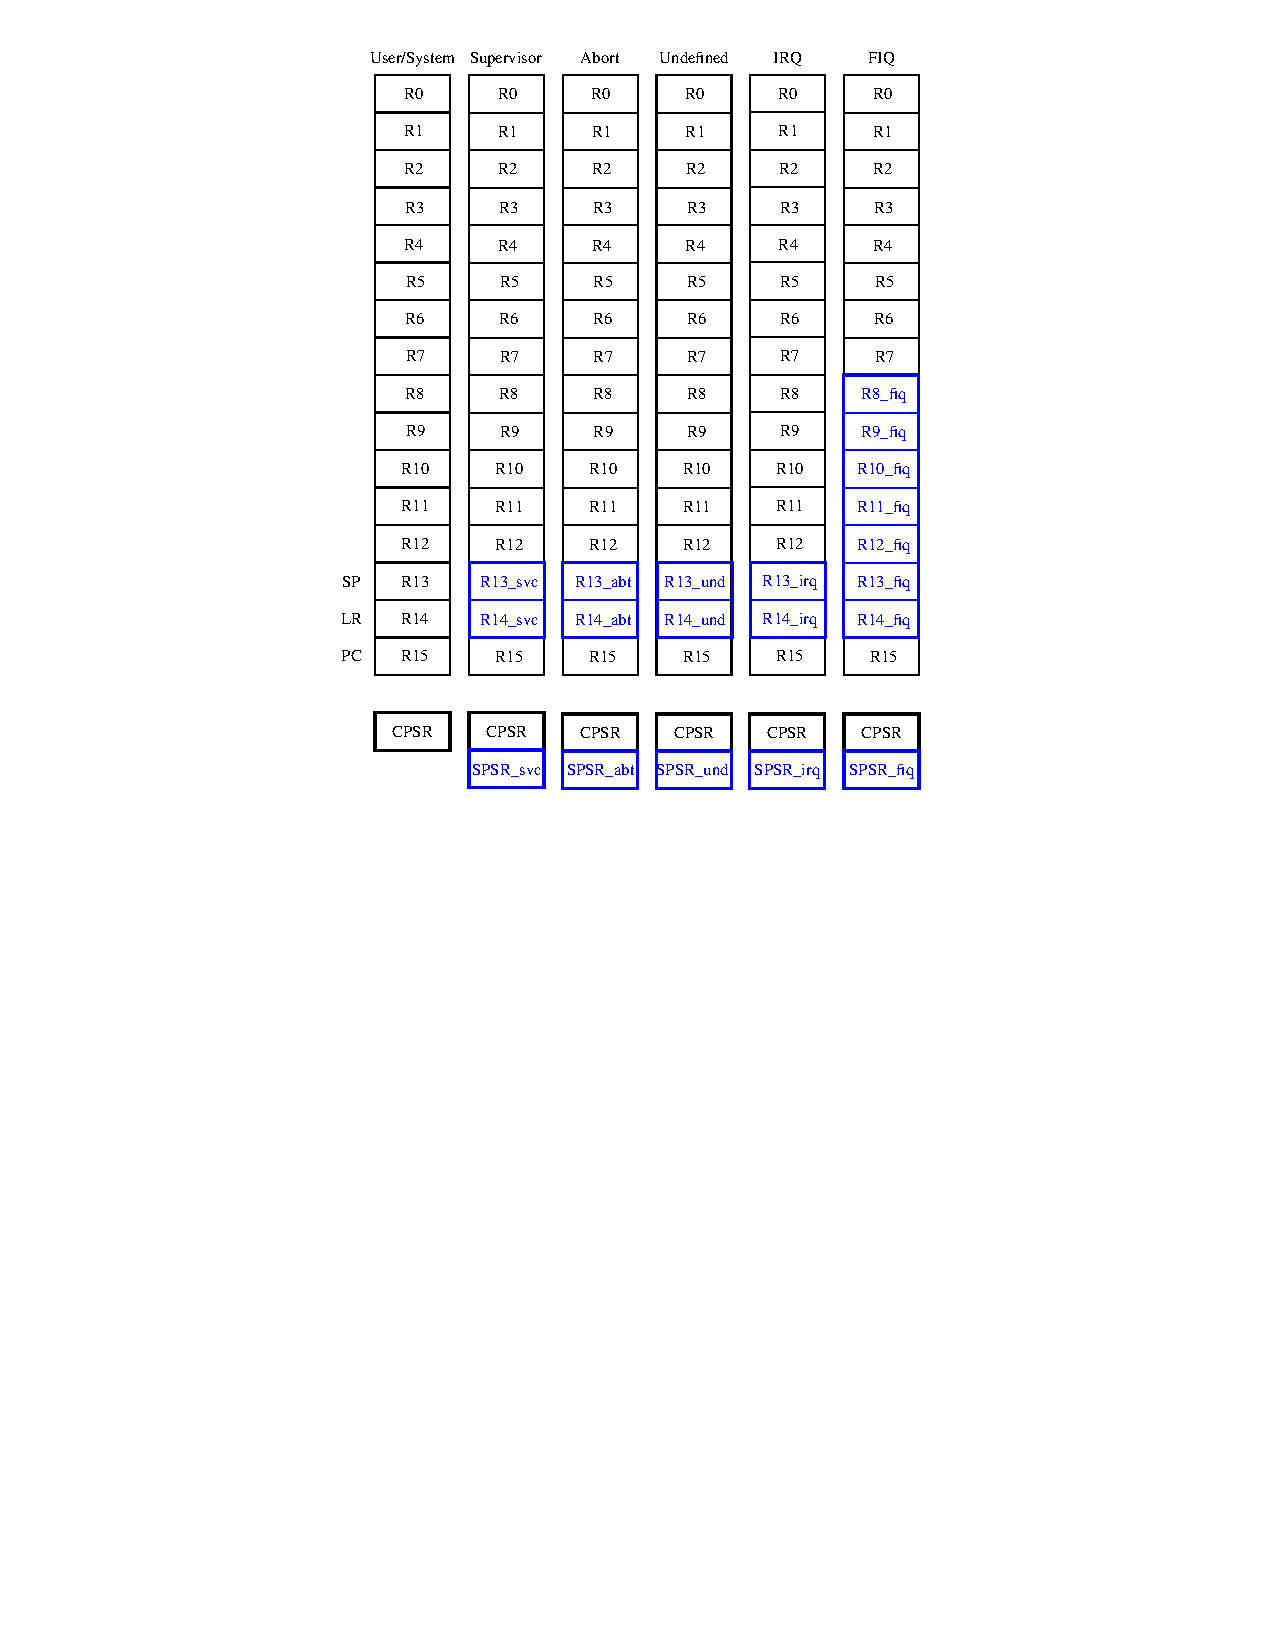
\includegraphics[scale=1]{figures/figure4.pdf}
   \caption{Registers used in various operating modes.} 
	 \label{fig:4}
	 \end{center}
\end{figure}

Note that registers R0 to R12 are not banked in most operating
modes. Thus, when an exception service routine needs to use some
of these registers, the contents of the registers must be saved
on the stack and later restored.
However, having the five banked registers R8\_fiq to R12\_fiq in
the FIQ mode, it is possible to respond very quickly to a fast
interrupt request if these registers are sufficient for the task
that is implemented by the corresponding interrupt-service
routine.

In Figure 4 and in the above discussion we referred to the
specific banked registers by appending a mode specifier, e.g.
R14\_svc. In an assembly-language program such specifiers are
not included, because the processor accesses the desired banked
register based on its current operating mode, as indicated by
the processor-mode bits, CPSR$_{4-0}$.  

In the Supervisor mode, the special Move instructions, MRS and
MSR, can be used to access the processor status registers CPSR
and SPSR\_svc.
The instruction
\begin{center}
MRS~~~R$d$, CPSR
\end{center}
\noindent
copies the contents of CPSR into register R$d$. Writing into
the status registers can be done by affecting one or more fields
of the register. The processor status registers have four fields of eight bits, identified by the field specifiers \_f, \_s, \_x and \_c, which correspond to PSR$_{31-24}$, PSR$_{23-16}$,
PSR$_{15-8}$ and PSR$_{7-0}$, respectively. Thus, the instruction
\begin{center}
MSR~~~CPSR\_c, R$d$
\end{center}
\noindent
copies the contents of R$d$ into CPSR$_{7-0}$, which affects only the processor mode and interrupt disable bits. All bits can be affected by the instruction
\begin{center}
MSR~~~CPSR\_cxsf, R$d$
\end{center}
\noindent
We should note that the field specifiers must be used in the
MSR instruction; otherwise, an error will occur at compile
time.

In an exception mode, such as IRQ, it is the banked saved
status register that is accessed. Thus,
\begin{center}
MRS~~~R$d$, SPSR
\end{center}
\noindent
copies the contents of SPSR\_irq into register R$d$.

\section{Exception Processing}
\label{sec:exceptions}

An {\it exception} in the normal flow of program execution can be caused by:
\begin{itemize}
\item Software interrupt
\item Hardware interrupt
\item Attempted accessing of a nonexistent memory location
\item Unimplemented instruction
\end{itemize}
\noindent
The ARM Cortex-A9 processor uses a vectored exception scheme, in
which there is a separate vector of information assigned to each
type of exception. This vector normally consists of an instruction
that loads into the program counter the address of the first
instruction of the corresponding exception-service routine. 
The vectors are stored 
in the {\it exception vector table} at pre-assigned locations.
Table 4 gives the assignment of exception vectors in the
exception vector table. It also shows the priority levels
for the various exceptions and the mode entered upon the
occurrence of an exception.

\newpage
\begin{center}
{\bf TABLE 4. ~Exception Vector Table}
\vs
\begin{tabular}{llll}
\hline
\vs
{\bf Address} & {\bf Exception} &  {\bf Priority} & {\bf Mode entered}\\
\vs
\hline
\vs
0x000 & Reset & 1 & Supervisor\\
0x004 & Unimplemented instruction & 6 & Undefined\\
0x008 & Software interrupt & $-$ & Supervisor\\
0x00C & Instruction access violation & 5 & Abort\\
0x010 & Data access violation & 2 & Abort\\
0x018 & IRQ & 4 & IRQ\\
0x01C & FIQ & 3 & FIQ\\
\vs
\hline
\end{tabular}
\end{center}

When an exception occurs in the User mode, the ARM processor
switches into the corresponding exception mode and automatically performs the following actions:
\begin{itemize}
\item Saves the contents of the Program Counter in the banked
Link register, LR\_mode.
\item Saves the contents of the processor status register, CPSR,
in the banked status register, SPSR\_mode.
\item Changes the mode bits in CPSR to denote the exception mode,
and sets the interrupt-disable bits, I and F, accordingly.
\item Loads the Program Counter, PC, with a vector
address for the exception that caused the action. At this address
in the exception table there is an instruction that is executed
next. 
\end{itemize}

\subsection{Software Interrupt}
\label{sec:SVC}

A software interrupt, which is called a {\it software exception}
in ARM literature, occurs when an SVC instruction is
encountered in a program. This instruction causes the processor
to switch into Supervisor mode.
The address of the next instruction is saved in the banked register LR\_svc and the contents of CPSR are saved in SPSR\_svc.
Then, the address of entry 8 in the exception vector table
is loaded into the Program Counter. A branch instruction at that
location leads to to the required exception-service routine.

Upon completion of the exception-service routine, a return to the
interrupted program can be realized with the instruction
\begin{center}
MOVS~~~PC, LR
\end{center}
\noindent
Note that the suffix S in the OP-code mnemonic normally specifies
that the Condition Code flags should be set. However, when the
destination register is PC, the suffix S causes the saved
contents in register SPSR\_mode, in this case SPSR\_svc, to 
be loaded into the processor status register CPSR. Since this
instruction also loads the saved return address into PC, a return
to the interrupted program is completed.

A common use of the software interrupt is to transfer control to
a different program, such as an operating system.

\subsection{Hardware Interrupts}
\label{sec:hardware_interrupts}

Hardware interrupts can be raised by external sources, such as
I/O devices, by asserting one of the processor's
interrupt-request inputs, IRQ or FIQ.
When the processor receives a hardware interrupt request, it
enters the corresponding exception mode to service the interrupt.
It also saves the contents of PC and CPSR. 

The saved contents of the PC are supposed to be the return
address. However, this is not the case with the ARM Cortex-A9
processor. This processor prefetches instructions for execution.
While the current instruction is being executed, the next
instruction is prefetched and its processing is started.
This means that the Program Counter points to the instruction
after the prefetched one. Namely, the updated contents of PC
are the address of the current instruction plus 8.
Since the interrupt is serviced upon completion of the current
instruction, the next prefetched instruction is discarded and
it must be executed upon return from the interrupt. Therefore,
the address saved in the link register must be decremented
by 4 prior to returning to the interrupted program.
This can be done by having
\begin{center}
SUBS~~~PC, LR, \#4
\end{center}
\noindent
as the last instruction in the exception-service routine.
Note that the suffix S causes a proper return to the interrupted
program, as explained above.

\subsubsection{IRQ Interrupts}
\label{sec:IRQ}

Upon accepting an IRQ interrupt request, the processor 
saves the contents of CPSR in the SPSR\_irq register, and
it saves the contents of PC in the link register LR\_irq.
It also sets the mode bits in CPSR to denote the IRQ exception
mode, and it sets the I bit to 1 to disable further IRQ
interrupts. Then, it executes the instruction at location
0x018 of the exception vector table, which has to cause
a branch that leads to the IRQ exception-service routine.

The return from the exception-service routine should be performed
with the instruction
\begin{center}
SUBS~~~PC, LR, \#4
\end{center}
\noindent

\subsubsection{FIQ Interrupts}

An FIQ interrupt request is raised by a device that needs fast
response. Upon accepting the request, the processor 
saves the contents of CPSR in the SPSR\_fiq register, and
it saves the contents of PC in the link register LR\_fiq.
It also sets the mode bits in CPSR to denote the FIQ exception
mode, and it sets the F and I bits to 1 to disable further
interrupts. Then, it executes the instruction at location
0x01C of the exception vector table. Since this is the last 
location in the exception vector table, it can actually hold
the first instruction of the FIQ exception-service routine
(instead of an instruction that causes a branch to the FIQ
exception-service routine), which speeds up the response to
the FIQ request.

In the FIQ mode there are five additional banked registers,
R8\_fiq to R12\_fiq, which means that the exception-service 
routine can use these registers without first having to save the 
contents of R8 to R12 on the stack. This leads to a faster
response.

The return from the exception-service routine should be performed
with the instruction
\begin{center}
SUBS~~~PC, LR, \#4
\end{center}
\noindent

\subsection{Unimplemented Instruction}

This exception occurs when the processor encounters a valid
instruction that is not implemented in hardware. 
The exception-service routine may emulate the required operation
in software.

The return from the exception-service routine should be performed
with the instruction
\begin{center}
SUBS~~~PC, LR, \#4
\end{center}
\noindent

\subsection{Instruction Access Violation}

This exception occurs if the processor tries to access an
instruction at a non-existing memory location.

The return from the exception-service routine should be performed
with the instruction
\begin{center}
SUBS~~~PC, LR, \#4
\end{center}
\noindent

\subsection{Data Access Violation}

This exception occurs if the processor tries to access data
at a non-existing memory location.

In this case, the return from the exception-service routine
should be performed with the instruction
\begin{center}
SUBS~~~PC, LR, \#8
\end{center}
\noindent

\subsection{Nested Interrupts}

When two or more interrupts or exceptions occur at different
priority levels, causing the processor to enter different
modes of operation, their servicing can proceed immediately
because the banked registers in various modes are used to save 
the critical information about the interrupted program.
However, if multiple interrupts can occur at the same priority
level, typically multiple IRQ requests, then it is necessary
to nest the exception-service routines. This includes saving
the contents of the banked link register, LR\_mode,
on the stack before enabling subsequent
requests. Before returning from the corresponding
exception-service routine, the contents of the register must
be restored.

\subsection{Exception Processing Example}

The following example shows how the exception vector table can be
set up, and how the exception-service routines can be organized.
We will use a hardware IRQ interrupt as an example of an
exception-service routine.

As shown in Table 4, the exception vector table must occupy
the fixed memory locations in the address range 0x000 to 0x01C.
Each word in this table must be an instruction that causes the
program execution to go to the corresponding exception-service
routine. This requires the program counter to be loaded with
the address of the first instruction in the exception-service
routine. This can be accomplished with load instructions
\begin{center}
LDR~~~~PC, =EXCEPTION\_SERVICE\_ROUTINE\_NAME
\end{center}
Figure 5 illustrates the structure of the code that can be used.

\begin{figure}[H]
\begin{center} %%%\begin{singlespace}
\begin{lstlisting}[style=defaultArmStyle]
        .text
        .global  _start
        LDR      PC, =_start              /* Go to the beginning of the MAIN */
                                          /* program. */
        LDR      PC, =SERVICE_UND         /* Unimplemented instruction. */
        LDR      PC, =SERVICE_SVC         /* Software interrupt. */
        LDR      PC, =SERVICE_ABT_INST    /* Failed instruction access. */
        LDR      PC, =SERVICE_ABT_DATA    /* Failed data access. */
        .word    0                        /* Null entry for address 0x014. */
        LDR      PC, =SERVICE_IRQ         /* Hardware IRQ interrupt. */
        LDR      PC, =SERVICE_FIQ         /* Hardware FIQ interrupt. */
				
/* The main program. */
_start: ...
        .
        .
        .
				
/* Service routine for IRQ interrupts. */
SERVICE_IRQ:
        .
        .
        .
        SUBS PC, LR, #4                    /* Return to interrupted program. */

/* Service routine for software interrupts. */
SERVICE_SVC:
        .
        .
        .
        MOVS PC, LR                        /* Return to interrupted program. */
	

\end{lstlisting} %%%\end{singlespace}
\end{center}
	\vspace{-0.33in}
	\caption{Code used to set up the exception processing.}
	\label{fig:5}
\end{figure}

Observe that 0x000 is inserted in address location 0x014,
because this vector location is not allocated to servicing an
exception. Observe also that the return from the
exception-service routines used as an example is done as
explained in sections \ref{sec:hardware_interrupts} and \ref{sec:IRQ}.

\section{Input/Output Operations}

Most I/O devices are accessed by means of their memory-mapped
registers. When a program accesses such devices, it is important
that each access is made to an actual register. In a
processor with a data cache, it is essential to ensure that the cached data is not used instead of the current values in the I/O device registers. In effect, the data cache has to be bypassed
when reading or writing the registers in I/O devices.
The ARM processor does not have separate instructions for reading
and writing the contents of I/O registers. Instead, all I/O
devices must have their registers mapped into a memory address
region that will not be cached by the processor. This can be accomplished if
the processor data cache is disabled completely, or if the processor's memory management
unit (MMU) is set up such that appropriate regions of memory are designated as non-cacheable. The 
procedure for setting up the MMU and data cache is beyond the scope of this document.

% Copyright and Trademark

%\newcommand{\datePublished}{Mar 2022}

\newcommand{\versnum}{21.1} %version number quartus/AMP
\newcommand{\quartusname}{Quartus\textsuperscript{\textregistered} Prime}	
\newcommand{\textBar}{For \quartusname{} \versnum{}}
\newcommand{\thisyear}{2022 } %for copyright
\newcommand{\company}{FPGAcademy.org}
\newcommand{\longteamname}{FPGAcademy.org}
\newcommand{\teamname}{FPGAcademy}
\newcommand{\website}{FPGAcademy.org}

\newcommand{\productAcronym}{AMP}
\newcommand{\productNameShort}{Monitor Program}

\newcommand{\productNameMedTM}{Monitor Program}
\newcommand{\productNameMed}{Monitor Program}

%\newcommand{\headerLogoFilePath}[1]{#1/FPGAcademy.png}



%%%%%%%%%%%%%%%%%%%%%%%%%%%%%%%%%%%%%%%%
%%% FPGAcademy Copyright Information %%%
%%%%%%%%%%%%%%%%%%%%%%%%%%%%%%%%%%%%%%%%

%Always put the copyright on a new page (clear page), with some vertical space from top
\clearpage
\vspace{1in}

\noindent

Copyright {\copyright} FPGAcademy.org. All rights reserved. FPGAcademy and the FPGAcademy logo are trademarks of  FPGAcademy.org.  This document is being provided on an ``as-is'' basis and as an accommodation and therefore all warranties, representations or guarantees of any kind (whether express, implied or statutory) including, without limitation, warranties of merchantability, non-infringement, or fitness for a particular purpose, are specifically disclaimed.

%FPGAcademy assumes no responsibility or liability arising out of the application or use of any information,  product,  or  service  described  herein  except  as  expressly  agreed  to  in  writing  by  FPGAcademy.



**Other names and brands may be claimed as the property of others.





\end{document}
